\documentclass[12pt]{article}
\usepackage[usenames,dvipsnames]{color}
\usepackage{listings}
\usepackage{graphicx}
\usepackage{fancyhdr}
\usepackage{framed}
\usepackage[T1]{fontenc}
\usepackage[toc,page]{appendix}
\usepackage[utf8]{inputenc}
\usepackage[brazil]{babel}
\usepackage{fancyvrb}
\usepackage[hmargin=2cm,vmargin=2cm]{geometry}
\usepackage{lastpage}
\usepackage{makeidx}
\pagestyle{fancy}

% cabecalho e rodapé
\setlength{\headheight}{120pt}
\setlength{\textheight}{550pt}
\renewcommand{\headrulewidth}{0pt}
\lhead{
\includegraphics[scale=0.03]{brasao.png}}
\rhead{
\includegraphics[scale=0.4]{logo-pnud.png}}
\cfoot{\textbf{\ProjectCode\ - Inovando a democracia participativa}}
\rfoot{\thepage}

\hyphenation{par-ti-ci-pa-ção}
\bibliographystyle{ieeetr}

% definições sobre o autor e o produto
\newcommand{\MyName}{Joenio Marques da Costa}
\newcommand{\MySurnameForename}{Costa, Joenio}
\newcommand{\SupervisorName}{Ricardo Augusto Poppi Martins}
\newcommand{\MyEmail}{joenio@colivre.coop.br}
\newcommand{\ContractNumber}{2013/000564}
\newcommand{\ContractYear}{2013}
\newcommand{\ProjectCode}{Projeto BRA/12/018}
\newcommand{\NomeSecretaria}{Secretaria Geral da Presidência da República}
\newcommand{\SiglaSecretaria}{SG/PR}
\newcommand{\ProductNumber}{06}
\newcommand{\ProductTitle}{Protocolos para federação de redes sociais}
\newcommand{\ProductSubtitle}{Proposta de federação entre o Participa.br e as
  redes Diaspora}
\newcommand{\ProductDescription}{"Documento com análise de protocolos,
  arquiteturas e sistemas de federação de conteúdos para ambientes de redes
  Sociais com estratégia de implantação considerando os sites parceiros e
  contendo propostas de códigos. Inclui especificações e códigos para conexão
  de contas e trocas de postagens do portal com redes sociais proprietárias."
}
\newcommand{\ProductValue}{R\$ 14.400,00 (quatorze mil e quatrocentos reais)}
\newcommand{\ObjetoContratacao}{"Construção dos códigos para comunidades e
  aplicativos do portal da participação social."
}
\newcommand{\DataEntrega}{25 Novembro de 2014}
\newcommand{\PalavrasChave}{federação, redes sociais, diaspora, descentralização}

% lista de abreviações
\makeindex

\begin{document}

\newgeometry{hmargin=3cm,vmargin=1.5cm}
\addtolength{\topmargin}{2.5cm}
\thispagestyle{empty}
{\color{MidnightBlue}

{\bf \LARGE Produto \ProductNumber\ -\ \ProductTitle}

\hrulefill

\vspace{1cm}

\begin{center}

{\bf \large Contrato n. \ContractNumber}

\vspace{1.5cm}

{\bf \large Objeto da contratação: \ObjetoContratacao}

\end{center}

\vspace{3.2cm}

Valor do produto: \ProductValue

\vspace{1.2cm}

Data de entrega: \DataEntrega

\vspace{1.2cm}

Nome do consultor: \MyName

\vspace{1.2cm}

Nome do supervisor: \SupervisorName

}

\vspace{2cm}

\begin{center}

\includegraphics[scale=0.04]{brasao.png} \\
{\bf \small \NomeSecretaria}
\end{center}

\restoregeometry
\newpage

\newgeometry{hmargin=3cm,vmargin=1.5cm}
\begin{center}
\thispagestyle{empty}
{\color{MidnightBlue}


\includegraphics[scale=0.9]{logo-pnud.png}

\vspace{4cm}

{\bf \large \ProjectCode\ - Desenvolvimento de Metodologias
de Articulação e Gestão de Políticas Públicas para Promoção da Democracia
Participativa}

\vspace{1.5cm}

{\bf \large Produto \ProductNumber\ -\ \ProductTitle}

\vspace{1.5cm}

\ProductSubtitle

\vspace{4cm}

\MyName

\vspace{2cm}

}


\includegraphics[scale=0.04]{brasao.png} \\
{\bf \small \NomeSecretaria}

\end{center}
\restoregeometry
\newpage

\newgeometry{hmargin=3cm,vmargin=1.5cm}
\addtolength{\topmargin}{2.5cm}
\thispagestyle{empty}
{\color{MidnightBlue}

{\bf \LARGE Produto \ProductNumber\ -\ \ProductTitle}

\hrulefill

\vspace{1cm}

\begin{center}

{\bf \large Contrato n. \ContractNumber}

\vspace{1.5cm}

{\bf \large Objeto da contratação: \ObjetoContratacao}

\end{center}

\vspace{3.2cm}

Valor do produto: \ProductValue

\vspace{1.2cm}

Data de entrega: \DataEntrega

\vspace{1.2cm}

Nome do consultor(a): \MyName

\vspace{1.2cm}

Nome do supervisor(a): \SupervisorName

}

\vspace{2cm}

\begin{center}

\includegraphics[scale=0.04]{brasao.png} \\
{\bf \small \NomeSecretaria}
\end{center}

\restoregeometry
\newpage

\newgeometry{hmargin=3cm,vmargin=1.5cm}
\addtolength{\topmargin}{5cm}
\thispagestyle{empty}

\begin{framed}

{\raggedright \MySurnameForename} \\

\ProductTitle: \ProductSubtitle\ / \ContractYear. \\

Total de folhas: \pageref{LastPage} \\

\vspace{1cm}

Supervisor: \SupervisorName \\

\SiglaSecretaria \\

\NomeSecretaria \\

Palavras-chave: \PalavrasChave. \\

\end{framed}

\vspace{3cm}

{\raggedright 
\includegraphics{licenca-cc-by-nc.png} \ Esta obra é licenciada sob
uma licença Creative Commons - Atribuição-NãoComercial. 4.0 Internacional.}

\restoregeometry
\newpage

\tableofcontents
\newpage

\begin{abstract}
... \\

{\bf Palavras-chave:} \PalavrasChave.
\end{abstract}
\newpage

\section{Introdução}

Em consonância com os objetivos e cronograma previsto no âmbito do
projeto BRA/12/018:
\textbf{Desenvolvimento de Metodologias de Articulação e Gestão de
Políticas Públicas para Promoção da Democracia Participativa},
firmado entre a Secretaria-Geral da Presidência da República
(SG/PR) e o Programa das Nações Unidas para o Desenvolvimento (PNUD),
o presente documento apresenta \ProductDescription.

Essa proposta está configurada como produto \ProductNumber~da consultoria técnica
para especificação da construção dos códigos das metodologias de
organização da informação e interação participativa do portal de
participação social.

\section{O Participa.br}

O Participa.br é a Plataforma Federal da Participação Social. Trata-se de mais
um espaço para participação social no Brasil, escuta e diálogo entre o Governo
Federal e a Sociedade Civil. 

A plataforma, totalmente desenvolvida em software livre, tem como missão
desenvolver práticas inovadoras de participação via internet e oferta de
espaços de manifestação e debate para qualquer cidadão ou organização, com o
intuito de construir políticas públicas cada vez mais eficazes e efetivas.

O Participa.br é desenvolvido sob a plataforma para redes sociais Noosfero.

\section{O Noosfero}

O Noosfero\cite{noosfero} é uma plataforma web livre para redes sociais e de
economia solidária que possui as funcionalidades de Blog, e-Portfolios, CMS,
RSS, discussão temática, agenda de eventos e inteligência econômica
colaborativa num mesmo sistema! O Noosfero utiliza a linguagem de programação
Ruby com framework Rails e, portanto, suporta bancos de dados, PostgreSQL,
MySQL, SQLite entre outros.

Noosfero é um Software Livre e licenciado sob a GNU Affero General Public
License (AGPL), versão 3.

\section{Redes sociais federadas}

Federação é a combinação de multiplos sistemas de computação funcionando sobre
padrões de operação compatíveis entre sí. Ou seja, sistemas com estruturas
internas diferentes funcionando em conjunto de forma transparente
\cite{federacao}.

Em sistemas em rede, federação significa que os usuários conseguem enviar
mensagens de um sistema a outro através da rede, sendo estes sistemas
distintos entre sí mas seguindo padrões de comunicação previamente definidos.

Exemplos de sistemas federados são inúmeros, dentre eles podemos citar
sistemas de email, chats Jabber, chats IRC, dentre outros. A maneira de
funcionamento de cada sistema é única, para cada serviço há uma proposta
diferente, sistemas de email por exemplo seguem o protocolo de envios de
mensagens chamado SMTP\cite{smtp} que é o responsável por garantir federação
no envio das mensagens. Desta forma um sistema federado de troca de
mensagens é independente de plataforma, ou seja, usuários de um fornecedor de
email (exemplo GMail) podem interagir de forma transparente com usuários de
outros fornecedores (exemplo Hotmail).

Chats Jabber por outro lado se baseiam no protocolo chamado XMPP\cite{xmpp},
com ele usuários podem usar serviços distintos e conversarem entre sí de forma
transparente. Chats IRC são implementados com base no protocolo de mesmo nome
chamado IRC\cite{irc}, exemplo de rede IRC em Figura \ref{irc}.

\begin{figure}[h]
\center
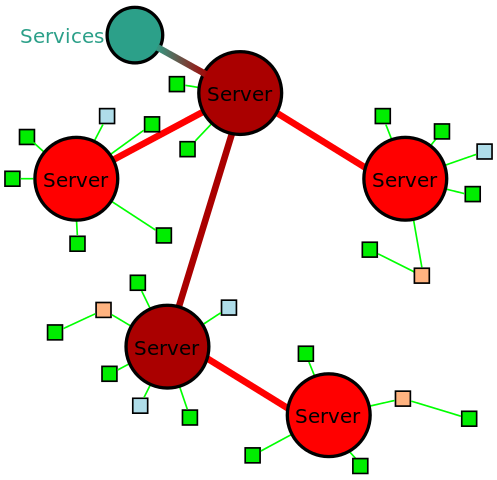
\includegraphics[scale=0.4]{Ircnetz-Schema.png}
\caption{Exemplo de rede federada IRC}
\label{irc}
\end{figure}
% fonte: https://pt.wikipedia.org/wiki/Ficheiro:Ircnetz-Schema.svg

Todos estes exemplos tem servido como inspiração para o desenvolveimento de
protocolos para federação de redes sociais, as principais redes sociais
modernas não são federadas, e são ainda extremamente centralizadas. Redes como
Facebook e Google Plus por exemplo obrigam os usuários estarem cadastrados em
sua base da dados para poderem interagir com os usuários e comunidades.

Um movimento para quebrar este paradigma de redes sociais extremamente
isoladas começou a surgir através do termo {\it redes sociais virtuais
federadas}, o termo {\it federada} foi usado em detrimento do termo {\it
aberta} para não causar confusão pois ela é mais específica e estabelece
claramente o que se pretende: criar redes sociais que se interconectem entre
sí de forma transparente. Este movimento foi iniciado em 2010 a partir de um
evento chamado {\it Federated Social Web Conference}\cite{aurelio}.

\section{Protocolos para federação de redes sociais}

Inúmeras iniciativas e propostas tem surgido para solucionar o isolamento das
redes sociais e promover interoperabilidade e descentralização, alguns
dos protocolos mais populares e comumente referenciados são listados a seguir.

\subsection{Activity Streams}

É uma especificação de formato aberto para um protocolo de {\it streaming} de
atividades, com foco em criar criar um consórcio entre aplicações e serviços
web, um {\it streaming} de atividades é algo similar a linha do tempo do
Facebook.

A maior implementação do protocolo é o Stream Framework\cite{stream}, uma
biblioteca em Python para construção de fonte de notícias usando Cassandra ou
Redis.

A especificação do protocolo\cite{streams} basicamente define um formato comum
para transmitir informações do tipo: "Geraldino postou uma foto em seu álbum"
ou "João compartilhou um vídeo".

\begin{itemize}
  \item http://en.wikipedia.org/wiki/Activity\_Streams\_(format)
\end{itemize}

\subsection{Diaspora's Federation Protocol}

O protocolo Diaspora descreve como deve ocorrer a comunicação entre servidores
Diaspora. O compartilhamento através deste protocolo é assimétrica, ou seja,
em um relacionamento um usuário inicia compartilhamento com alguém, mesmo que
esse alguém nao deseje compartilhar com você. Desta forma um usuário pode
compartilhar tudo com um outro certo usuário que não deseje compartilhar nada
com ele. O envio de postagens é feito através do protocolo Salmon.

\begin{itemize}
  \item https://wiki.diasporafoundation.org/Federation\_Protocol\_Overview
\end{itemize}

\subsection{FOAF}

FOAF é uma ontologia para descrição de pessoas com foco em fácil leitura por
máquinas, suas ativiades e seus relacionamentos. Qualquer um pode usar FOAF
para descrever a sí mesmo. Permite grupos de pessoas descrever redes sociais
sem necessidade de um banco de dados centralizado.

É um vocabulário descritivo espressado em RDF e OWL, computadores podem
usar os perfis FOAF para encontrar, por exemplo, todas as pessoas vivendo na
Europa, ou para listar todas as pessoas que são amigas de alguém. Cada perfil
tem um identificador único usado para definir estas relações.

O projeto foi iniciado em 2000 e pode ser considerado a primeira aplicação da
Web Semantica, que combina tecnologia RDF com conceitos da 'Web Social'.

\begin{itemize}
  \item http://en.wikipedia.org/wiki/FOAF\_(ontology)
\end{itemize}

\subsection{Google Wave Federation Protocol}

O protocolo Wave Federation é um protocolo aberto, uma extensão do XMPP, usado
no Apache Wave. Projetado para comunicação em tempo real através de servidores
trabalhando de forma cooperativa.

Ainda em desenvolvimento ativo, o protocolo é fortemente baseado no protocolo
de email e as funcionalidades inplementadas em cima dele são formetemte
guiadas pela idela de email.

Java source code for the "Google Wave Federation Prototype Server" was
released in a Mercurial repository in July 2009 under the Apache License
2.0.[6][7]

\begin{itemize}
  \item http://en.wikipedia.org/wiki/Google\_Wave\_Federation\_Protocol
\end{itemize}

\subsection{OStatus}

OStatus é um padrão aberto para compartilhamento de atualizações que faz
referencias a protocolos abertos como Atom, Activity Streams, PubSubHubbub,
Walmon, Webfinger, que permitem pontos de troca e roteamento de mensagens e
atualizações de status entre usuários em tempo real.

Federação com OStatus foi inicialmente implementado no StatusNet e
posterioemente em MiniMe, um projeto de microblog. Em janeiro de 2012 o W3C
adotou e passou a manter o OStatus.

\begin{itemize}
  \item http://en.wikipedia.org/wiki/OStatus
\end{itemize}

\subsection{OpenSocial}

OpenSocial é uma especificação pública que define um componente de hospedagem
e um conjunto de APIs para aplicações web. Iniciamente projetado para
aplicações de redes sociais foi desenvolvido pelo Google e MySpace e outras
redes sociais. a OpenSocial Foundation suporta várias outras tecnologias Web
como OAuth, Activity Streams e Portable Contacts.

Foi lançado em Novembro de 2007, aplicações que implementam as APIs do
OpenSocial potem interoperar com qualquer outra rede social que suporta ele.

\begin{itemize}
  \item http://en.wikipedia.org/wiki/OpenSocial
\end{itemize}

\subsection{PubSubHubbub}

PubSubHubbub é um protocolo aberto para comunicação distribuída de
publicar/subscrever via Internet. Inicialmente projetado para extender os
protocolos Atom (e RSS) para feed de dados, o protocolo pode ser aplicado para
qualquer tipo de dado (texto, imagens, audio, vídeos) desde que estejam
disponívels via HTTP.

O principal objetivo é prover notificações de mudanças em tempo real. É
utulizado para empurrar conteúdo de muitos sites, como blogger.com,
wordpress.com, CNN, Fox News, diaspora*, entre outros.

\begin{itemize}
  \item http://en.wikipedia.org/wiki/PubSubHubbub
\end{itemize}

\subsection{Pump.io}

Pump.io é um motor de activity streams de propósito geral que pode ser usado
como protocolo de rede social federada que "faz o que a maioria das pessoas
realmente precisam de uma rede social". Iniciado por Evan Prodromou, é uma
evolução do StatusNet. Identi.ca que foi um grande exemplo de uso do StatusNet
foi migrado para usar o pump.io desde 2013. Entretanto, enquanto o StatusNet
oferece serviço similar o Twitter, pump.io oferece recursos muito mais gerais
de rede social, e tem sido aditado por outros tipode de aplicação, como o
MediaGoblin.


\begin{itemize}
  \item http://en.wikipedia.org/wiki/Pump.io
\end{itemize}

\subsection{Salmon}

O protocolo Salmon é um protocolo para troca de mensagens sob HTTP projetado
para descentralizar comentários e anotações feitas em artigos como posts de
blogues. Permite threads de discussões serem feitas entre a origem do artigo e
o "agregador" que está inscrito e obtendo o conteúdo. De forma simples, um
artigo que aparece em 3 sites A (fonte original), B e C, membros dos 3
serviços podem contribuir com uma thread única de conversação.

Redes sociais federadas como StatusNet e Diaspora usam Salmon como definido na
especificação do OStatus para coordenar discussão entre membros de diferentes
servidores. Um membro de um servidor pode publicar um artigo que será
disseminado para outros usuários da rede via Salmon que em "turno" podem
comentar de volta de maneira transparente.

\begin{itemize}
  \item http://en.wikipedia.org/wiki/Salmon\_(protocol)
\end{itemize}

\subsection{Tent}

Tent é um protocolo para redes sociais abertas e descentralizadas. Usa
compartilhamento de conteúdos com aplicativos entre si. Qualquer um pode
executar um servidor Tent, ou escrever um aplicativo alternativo que use o
protocolo Tent. Usuários podem ter o controle do conteudo e relacionamentos
alterando ou movendo servidores. Tent suporta uma lista extensiva de tipos de
dados, desenvolvedores podem criar novos tipos de interação.

\begin{itemize}
  \item http://en.wikipedia.org/wiki/Tent\_(protocol)
\end{itemize}

\subsection{Webfinger}

Protocolo especificado pelo IETF que permite descobrir informações sobre
pessoas e coisas identificados por URI. Informações sobre uma pessoa pode ser
descoberta via um endereço "acct:", por exemplo um endereço similar a um
email.

É usado por redes como StatusNet e Diaspora para descobrir usuário em nós
federados e "pods" em protocolos de armazenamento remoto como ownCloud por
exemplo.

Historicamente foi derivado do Finger protocolo, mas é bem diferente por ser
projetado sob o HTTP.

\begin{itemize}
  \item http://en.wikipedia.org/wiki/WebFinger
\end{itemize}

http://noosfero.org/Development/ActionItem1573
This is the first real step to interact with diaspora and other federated networks.
Working branch: https://gitlab.com/aurium/noosfero/commits/init-federation

\section{Ferramentas de redes sociais federadas}

Estes protocolos isoladamente não fornecem solução para descentralizar as
redes e promover federação, é preciso ferramentas que implementem tais
protocolos, comumente mais de um protocolo é implementado nas ferramentas
atuais, cada protocolo atinge um problema específico, então a combinação deles
resulta num produto abrangente que resolve o problema mencionado. Segue
algumas ferramentas mais populares que implementam alguns dos protocolos
acima.

\subsection{Diaspora}

Diaspora é projetado para atacar problemas relacionados a privacidade em redes
sociais centralizadas permitindo os usuários subirem seu próprio servidor
(chamado "pod") para hospedar conteúdo. "pods" podem interagir para
compartilhar atualização de status, fotos e outros tipos de conteúdo. Isto
permite aos usuários hospedarem em um servidor dedicado ou compartilhado, é
implementado em Ruby on Rails e é software livre.

Uma parte central do software Diaspora é o conceito que ele deve agir como um
"agregador social", permitindo posts serem facilmente importados do Facebook,
Tumblr e Twitter. A ideia é que as barreiras legais para juntar as redes e
quanto mais amigos entrarem, você nao mais precisará do Facebook para se
comunicar. Ao invés disso, você poderá se comunicar, diretamente, de forma
segura, sem intermediários inescupulosos.

O software Diaspora implementa seu proprio protocolo de mesmo nome chamado
Diaspora, alem do WebFinger, Salmon, Activity Stream e o micro-formato h-card.

\begin{itemize}
  \item http://en.wikipedia.org/wiki/Diaspora\_(software)
\end{itemize}

\subsection{Friendica}

Friendica é um software livre que implementa uma rede social distribuída.
Possui enfase extensiva em configurações de privacidade e facilidade de
instalação em servidores. Tem objetivo de suportar federação com quantas
outras redes possível. Em novembro de 2014, o diretório global de usuários do
Friendica contabiliza 10 mil registros. Este é o número de usuários que
decidiram publicar seus perfis no diretório público global.

Implementa quais protocolos exatamente?

\begin{itemize}
  \item http://en.wikipedia.org/wiki/Friendica
\end{itemize}

\subsection{StatusNet / GNU Social}

GNU Social, também chamado de StatusNet, é um servidor de microblog livro
escrito em PHP que implementa o padrão OStatus para interoperação entre
instalações. Enquanto oferece funcionalidade similar ao Twitter, StatusNed
tenta prover o potencial para promover comunicação entre comunidades de
microblog abetras e distribuídas.

Implementa quais protocolos exatamente?

\begin{itemize}
  \item http://en.wikipedia.org/wiki/GNU\_social
\end{itemize}

\section{Federação entre o Participa.br e Diaspora}

Dentre os softwares citados anteriormente o Diaspora foi escolhido como um
plano piloto para ser integrado ao Participa.br, será descrito como o Diaspora
funciona em detalhes mais tecnicos, quais os passos para integrar o
Participa.br a ele, e então como integrar outras redes similar ao Participa.br
que também usem Noosfero, como por exemplo: Softwarelivre.org, Blogoosfero.cc,
Participa.gov.br, Juventude, etc...

\subsection{Diaspora em detalhes}

 * pesquisa o protocolo do diaspora
 * detalhes sobre este protocolo
 * nível de maturidade, aceitação e adoção

O Diaspora é tanto uma implamentação de uma ferramenta de rede social, quanto
uma especificação de protocolo para federação de redes sociais.
A implementação suporta as seguintes funcionalidades:

\begin{itemize}
  \item Status messages
  \item blogging
  \item photo sharing
  \item privacy enhanced
\end{itemize}

É implementado em Ruby on Rails e licenciado sob a licença
AGPL, implementa os protocolos:

\begin{itemize}
  \item Salmon
  \item WebFinger
  \item Activity Stream
  \item h-card
\end{itemize}

Utiliza as seguintes extensões junto ao Ruby on Rails, HAML, SASS, Backbone.js
e Handlebars.js. O banco de dados é organizado conforme os modelos abaixo:

\begin{itemize}
  \item User - Representação de um usuário no banco de dados
  \item Person - A representação de um usuário para o mundo exterior
  \item Contact - Define relações entre pessoas
  \item Request - Requisição de amizade entre pessoas
  \item Aspect - Uma lista de pessoas e postagens
  \item Post - Uma postagem associada a uma pessoa
\end{itemize}

Postando algo:

* Quando um usuário posta algo, ele posta isso em um ou vários Aspect
* Assumindo que o post é válido, é criado e armazenado em {\it raw\_visible\_posts}
* O HTML deste post é renderizado no servidor e enviado para o usuário via websocket
* O post é então serializado para XML e assinado em um envelope Salmon

\begin{framed}
\begin{lstlisting}[caption=Exemplo envio de mensagem e como o Diaspora serializa para XML]
  post.to_diaspora_xml
      def push_to_people(post, people)
        salmon = salmon(post)
        people.each{|person|
          xml = salmon.xml_for person
          push_to_person( person, xml)
        }
      end
  
  Salmon::SalmonSlap.create
      def self.create(user, activity)
        salmon = self.new
        salmon.author = user.person
        aes_key_hash = user.person.gen_aes_key
        salmon.aes_key = aes_key_hash['key']
        salmon.iv      = aes_key_hash['iv']
        salmon.magic_sig = MagicSigEnvelope.create(user,
          user.person.aes_encrypt(activity, aes_key_hash))
        salmon
      end
\end{lstlisting}
\end{framed}

Recebendo um post:

* O usuário recebe um Salmon, desencripta os cabeçalhos
* Se a assinatura do Salmon é válida ele é desempacotado e salvo no banco de dados
* Este post é armazenado entre os posts visiveis

\subsection{Integração entre Participa.br e o Diaspora}

 * proposta de como integrar o Noosfero as redes existentes Diaspora*
 * propoe integração do noosfero com ele

Para possibilitar integração entre o Participa.br e o Diaspora é preciso
implementar no Noosfero, software por trás do Participa.br, o suporte aos
protocolos utilizados no Diaspora, ou seja, implementar: Salmon, Activity
Stream, WebFinger, h-card e o proprio protocolo Diaspora.

\subsubsection{WebFinger e Noosfero}

Protocolo para descoberta de informações sobre pessoas e coisas identificados
por URI únicas. Ele é o primeiro passo para ter intereção real com o Diaspora
e outras redes sociais federadas.

O Noosfero não tem suporte a tal protocolo, mas houve uma iniciativa pessoal
de um dos desenvolvedores de documentar algo sobre este protocolo e iniciar
uma implementação:

\begin{itemize}
  \item Issue sobre WebFinger no tracker do Noosfero: \\
    http://noosfero.org/Development/ActionItem1573
  \item Branch no Git com a implementação parcial para WebFinger: \\
    https://gitlab.com/aurium/noosfero/commits/init-federation
\end{itemize}

O que precisa ser feito para finalizar o suporte?

\subsubsection{Salmon e Noosfero}

O protocolo Salmon é um protocolo para troca de mensagens sob HTTP projetado
para descentralizar comentários e anotações feitas em artigos como posts de
blogues.

O Noosfero não tem qualquer implementação ou iniciativa de implementar Salmon,
este protocolo é necessário ser implementado e para isso é preciso seguir os
seguintes passos: Implementar funçoes de "aggregator" no Noosfero.

O Noosfero deve ser capaz de ser um "aggregator" para ler um feed Salmon
localizado no lado Diaspora. Quando um usuário do lado do Noosfero deixa um
comentário neste feed, o Noosfero deve armazenar o comentário de forma usual,
e então realizar um requisição POST\cite{salmon} seguindo a versão Salmon da fonte do feed.

Esta requisição post tem o seguinte formato:

\begin{framed}
\begin{lstlisting}[caption=Exemplo requisição POST Salmon]
POST /salmon-endpoint HTTP/1.1
Host: example.org
Content-Type: application/atom+xml

<?xml version='1.0' encoding='UTF-8'?>
<me:env xmlns:me="http://salmon-protocol.org/ns/magic-env">
    <me:data type='application/atom+xml'>
    PD94bWwgdmVyc2lvbj0nMS4wJyBlbmNvZGluZz0nVVRGLTgnPz4KPGVudHJ5IH
    dodHRwOi8vd3d3LnczLm9yZy8yMDA1L0F0b20nPgogIDxpZD50YWc6ZXhhbXBs
    MjAwOTpjbXQtMC40NDc3NTcxODwvaWQ-ICAKICA8YXV0aG9yPjxuYW1lPnRlc3
    BsZS5jb208L25hbWUPHVyaT5hY2N0OmpwYW56ZXJAZ29vZ2xlLmNvbTwvdXJpP
    G9yPgogIDx0aHI6aW4tcmVwbHktdG8geG1sbnM6dGhyPSdodHRwOi8vcHVybC5
    uZGljYXRpb24vdGhyZWFkLzEuMCcKICAgICAgcmVmPSd0YWc6YmxvZ2dlci5jb
    TpibG9nLTg5MzU5MTM3NDMxMzMxMjczNy5wb3N0LTM4NjE2NjMyNTg1Mzg4NTc
    hZzpibG9nZ2VyLmNvbSwxOTk5OmJsb2ctODkzNTkxMzc0MzEzMzEyNzM3LnBvc
    TY2MzI1ODUzODg1Nzk1NAogIDwvdGhyOmluLXJlcGx5LXRvPgogIDxjb250ZW5
    vbiBzd2ltIHVwc3RyZWFtITwvY29udGVudD4KICA8dGl0bGUU2FsbW9uIHN3aW
    JlYW0hPC90aXRsZT4KICA8dXBkYXRlZD4yMDA5LTEyLTE4VDIwOjA0OjAzWjwv
    ZD4KPC9lbnRyeT4KICAgIA
    </me:data>
    <me:encoding>base64url</me: <me:alg>RSA-SHA256</me:alg>
    <me:sig>
    EvGSD2vi8qYcveHnb-rrlok07qnCXjn8YSeCDDXlbhILSabgvNsPpbe76up8w63i2f
    WHvLKJzeGLKfyHg8ZomQ
    </me:sig>
</me:env>
\end{lstlisting}
\end{framed}

Com o suporte ao Salmon completo no Noosfero, o Noosfero será capaz de ao
receber comentários em posts de blogs, notícias e afins, que estes comentários
sejam compartilhados com usuários em redes Diaspora.

\subsubsection{Activity Stream e Noosfero}

Activity Streams é uma especificação de formato aberto para um protocolo de
{\it stream} de atividades, usado para criar consórcio entre aplicações e
serviços web, similar a Linha do tempo do Facebook. Com ele é possível ter um
padrão comum de comunicação para troca de dados relaciodos ao conteúdo de uma
linha do tempo.

O Noosfero não tem suporte a este protocolo e precisa que seja implementado
como sugere a especificação do mesmo, basicamente uma atividade consiste de um
ator, um verbo, um objeto e um alvo. Ele conta a história de uma pessoa
realizando ações em um objeto, exemplo: "Geraldine postou uma foto em seu
album" ou "João compartilhou um video"\cite{streams}. Na maioria dos casos
estes componentes serão explícitos, mas eles podem ser imlicitos.

\begin{framed}
\begin{lstlisting}[caption=Exemplo simples de atividade JSON serielizada]
  {
    "published": "2011-02-10T15:04:55Z",
    "actor": {
      "url": "http://example.org/martin",
      "objectType" : "person",
      "id": "tag:example.org,2011:martin",
      "image": {
        "url": "http://example.org/martin/image",
        "width": 250,
        "height": 250
      },
      "displayName": "Martin Smith"
    },
    "verb": "post",
    "object" : {
      "url": "http://example.org/blog/2011/02/entry",
      "id": "tag:example.org,2011:abc123/xyz"
    },
    "target" : {
      "url": "http://example.org/blog/",
      "objectType": "blog",
      "id": "tag:example.org,2011:abc123",
      "displayName": "Martin's Blog"
    }
  }
\end{lstlisting}
\end{framed}

\subsubsection{Diaspora e Noosfero}

O protocolo Diaspora descreve como deve ocorrer a comunicação entre servidores
Dispora, está em versão Alpha e em constante evolução.

* Compartilhar notificações
* Des-compartilhar notificações
* Atualização de status
* Comentários em atualização de status
* Curtir em atualizações de status

https://wiki.diasporafoundation.org/Federation\_message\_semantics

\subsubsection{h-card e Noosfero}

h-card is a simple, open format for publishing people and organisations on the web. h-card is one of several open microformat draft standards suitable for embedding data in HTML/HTML5.

h-card is the microformats2 update to hCard.

\begin{framed}
\begin{lstlisting}[caption=Exemplo de h-card]
<p class="h-card">
  <img class="u-photo" src="http://example.org/photo.png" alt="" />
  <a class="p-name u-url" href="http://example.org">Joe Bloggs</a>
  <a class="u-email" href="mailto:joebloggs@example.com">
    joebloggs@example.com
  </a>, 
  <span class="p-street-address">17 Austerstrti</span>
  <span class="p-locality">Reykjavik</span>
  <span class="p-country-name">Iceland</span>
</p>
\end{lstlisting}
\end{framed}

Será preciso implementar h-card para os perfils de usuários do Noosfero,
apesar do Noosfero não suportar h-card diretamente, há algum suporte para
vCards, uma especificação mais ampla onde o h-card se insere, os arquivos do
Noosfero que precisam ser verificados e extendidos para adicionar suporte a
h-card são:

\begin{itemize}
  \item app/views/blocks/profile\_info.html.erb
  \item app/views/blocks/profile\_image.html.erb
  \item app/helpers/application\_helper.rb
  \item app/views/comment/\_comment\_actions.html.erb
\end{itemize}

O h-card é o formato onde os dados de cada perfil de usuário será publicado
para que outras redes leiam e obtenham informações sobre o usuário.

\subsection{Integração de redes Noosfero entre sí}

 * integração e entre os noosferos usando o mesmo protocolo

\section{Federação entre o Participa.br e Redes Sociais Proprietárias}

% Inclui especicações e códigos para conexão de contas e trocas de postagens do
% portal com redes sociais proprietárias.

\section{Conclusão}

Neste documento foi apresentado um \ProductDescription

%
% resumir a contribuição prática para o participa e seus usuários aqui
%

Lembramos que para tornar o Portal de Consulta Pública realmente um canal de
consulta e participação popular na discussão e na definição da agenda
prioritária do país, é necessário que além de documentação faça-se um esforço
de movimentar as pessoar fora do ambiente virtual, para que haja um
engajamento no uso e contribuição deste projeto de forma consistente e perene.

\newpage
\bibliography{bibliografia}
\newpage
\listoffigures
\newpage
\printindex
\newpage
\definecolor{lightgrey}{rgb}{0.95,0.95,0.95}
\lstset{language=Ruby,basicstyle=\small\ttfamily,backgroundcolor=\color{lightgrey}}

\section{Anexos}

\subsection{Exemplo de código do plugin Noosfero para pairwise}

\lstinputlisting{pairwise_content.rb}

\subsection{Exemplo de código XML retornado pelo pairwise-api}

\begin{lstlisting}
<?xml version="1.0" encoding="UTF-8"?>
<prompt>
  <created-at type="datetime">2010-07-01T23:48:01+00:00</created-at>
  <id type="integer">1</id>
  <left-choice-id type="integer">10</left-choice-id>
  <question-id type="integer">7</question-id>
  <right-choice-id type="integer">9</right-choice-id>
  <tracking nil="true"></tracking>
  <updated-at type="datetime">2010-07-01T23:48:01+00:00</updated-at>
  <votes-count type="integer">0</votes-count>
  <left-choice-text>bar</left-choice-text>
  <right-choice-text>foo</right-choice-text>
</prompt>
\end{lstlisting}

\newpage
\appendix
\appendixpage
\section{Foo bar}
\label{foobar}

%\lstinputlisting{observatorio.rb}


\end{document}
